\begin{enumerate}[label=\thesubsection.\arabic*.,ref=\thesubsection.\theenumi]
\numberwithin{equation}{enumi}

\item Consider an op amp having a single pole open loop response $G_{o} = 10^5$ and $f_{p} = 10$ Hz.Let op amp be ideal connected in non-inverting terminal with a nominal low frequency of closed loop gain of 100 
\subitem A manufacturing error introducing a second pole at $10^4$ Hz.Find the frequency at which $|GH| = 1$ and phase margin
\subitem What values of H phase margin is greater than 45\degree

\begin{figure}[ht!]
	\begin{center}
		\resizebox{\columnwidth/1}{!}{\tikzset{
        block/.style = {draw, rectangle,
            minimum height=1cm,
            minimum width=2cm},
        input/.style = {coordinate,node distance=1cm},
        output/.style = {coordinate,node distance=4cm},
        arrow/.style={draw, -latex,node distance=2cm},
        pinstyle/.style = {pin edge={latex-, black,node distance=2cm}},
        sum/.style = {draw, circle, node distance=1cm},
}

\begin{tikzpicture}[node distance=2.5cm,auto,>=latex']
  \node [input, name=input] {};
  \node [sum, right of=input] (sum) {};
  \node [block, right of = sum] (block1) {$G_c(s)$};
  \node [block, right of = block1] (block2) {$G(s)$};
  \node [output, right of= block2] (output) {};
  \draw [->] (input) -- node {$R(s)\ +$} (sum);
  \draw [->] (sum) -- node {} (block1);
  \draw [->] (block1) -- node {} (block2);
  \draw [->] (block2) -- node [name =y] {$Y(s)$} (output);
  \draw [->] (y) -- ++ (0,-2) -| node [pos=0.99] {$-$} (sum);
\end{tikzpicture}}
	\end{center}
	\caption{}
	\label{fig:ee18btech11034_fig}
\end{figure}

\solution Part 1 of the question
For a two-pole amplifier open loop transfer function is 

\begin{align}
    G\brak{s} = \frac{G_{o}}{\brak{1+\frac{s}{\omega_{1}}}\brak{1+\frac{s}{\omega_{2}}}}
\end{align}
Poles are at $f_{1} =10$ and $f_{2} = 10^{4}$
\begin{align}
G\brak{f} = \frac{G_{o}}{\brak{1+\j\frac{f}{f_{1}}}\brak{1+\j\frac{f}{f_{2}}}}
\\
\implies \frac{10^{5}}{\brak{1+\j\frac{f}{10}}\brak{1+\j\frac{f}{10^{4}}}}
\label{eq:ee18btech11034_1}
\end{align}
As given closed loop gain is 100
\begin{align}
    \abs T = 100
\end{align}
For nominal low frequency $|GH| \gg 1$ and from Fig.\ref{fig:ee18btech11034_fig}
\begin{align}
    T = \frac{G}{1+GH}
    \\
\implies \approx \frac{1}{H}
\end{align}
So from this 
\begin{align}
    H = 0.01
    \label{eq:ee18btech11034_2}
\end{align}
For the $|GH| = 1$ and from \eqref{eq:ee18btech11034_1} and \eqref{eq:ee18btech11034_2}
\begin{align}
   \frac{10^{3}}{\brak{\sqrt{1+\frac{f^2}{100}}}\brak{\sqrt{1+\frac{f^2}{10^{8}}}}} = 1
\end{align}
\begin{align}
    \brak{1+\frac{f^2}{100}}\brak{1+\frac{f^2}{10^{8}}} = 10^{6}
\end{align}
Solving f using python code  
\begin{align}
    f = 7861.5 
\end{align}
From definition of phase margin $\alpha = 180\degree + \phi$
where $\phi$ is the phase of GH
\begin{align}
\phi = -\tan^{-1}\brak{\frac{f}{10}} -\tan^{-1}\brak{\frac{f}{10^{4}}}
\label{eq:ee18btech11034_phaseGH}
\end{align}
At $f = 7861.5$
\begin{align}
    \phi = -128.1\degree
    \\
    \implies \alpha = 180\degree + \phi
    \label{eq:ee18btech11034_3}
    \\
    \implies \alpha = 51.9\degree
\end{align}
\textbf{Hence for frequency $f = 7861.5$ Hz $|GH| = 1$ and phase margin is 51.9\degree}

The following code for bode plot of part 1
\begin{lstlisting}
codes/ee18btech11034/ee18btech11034_1.py
\end{lstlisting}

\item Verification using Bode plot of part 1
\begin{figure}[!h]
\centering
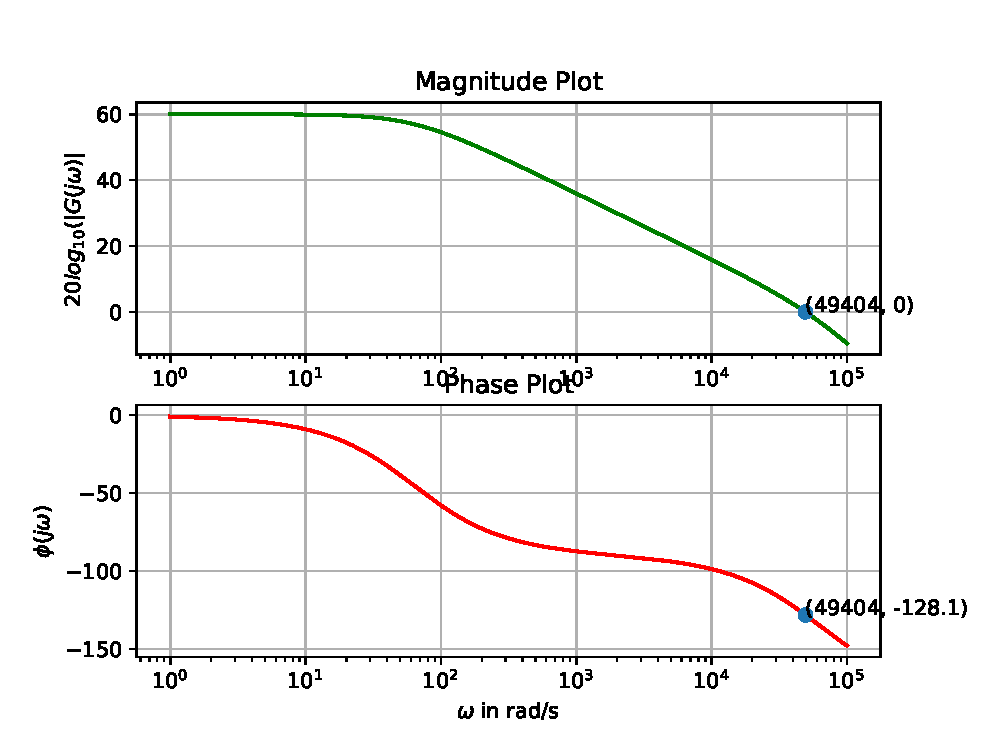
\includegraphics[width=\columnwidth]{./figs/ee18btech11034/ee18btech11034_1.eps}
\caption{}
\label{fig:ee18btech11034_1}
\end{figure}

\solution Part 2 of the question
For phase margin $\alpha=45\degree$ and from \eqref{eq:ee18btech11034_3}
\begin{align}
    \phi = -135\degree
    \label{eq:ee18btech11034_4}
\end{align}
From \eqref{eq:ee18btech11034_phaseGH} and \eqref{eq:ee18btech11034_4}
\begin{align}
    \phi = -\tan^{-1}\brak{\frac{f}{10}} -\tan^{-1}\brak{\frac{f}{10^{4}}}  = -135\degree
 \end{align}
 \begin{align}
\tan^{-1}\brak{\frac{\frac{f}{10} + \frac{f}{10^{4}}}{1-\frac{f^2}{10^{5}}}} = 135\degree
\end{align}
\begin{align}
    \frac{\frac{f}{10} + \frac{f}{10^{4}}}{1-\frac{f^2}{10^{5}}} = -1
\end{align}
Solving f using python
\begin{align}
    f \approx 10^{4}
\end{align}
For the above f equating $|GH|=1$ and from \eqref{eq:ee18btech11034_1}
\begin{align}
    \frac{\brak{10^{5}}H}{\brak{\sqrt{1+\frac{10^{8}}{100}}}\brak{\sqrt{1+\frac{10^{8}}{10^{8}}}}} = 1
\end{align}
Solving H using python code
\begin{align}
    H = 1.414 \times 10^{-2}
    \\
    \implies H_{max} =  1.414 \times 10^{-2}
\end{align}
In the part 1 of question for $H = 0.01$ which is less than $H_{max}$ phase margin is greater than 45\degree

So for 
\begin{align}
    H < H_{max} 
    \\
    \implies H < 1.414 \times 10^{-2}
\end{align}
the phase margin is greater than 45\degree

The following code for bode plot of part 2
\begin{lstlisting}
codes/ee18btech11034/ee18btech11034_2.py
\end{lstlisting}

\item Verification using Bode plot of part 2
\begin{figure}[!h]
\centering
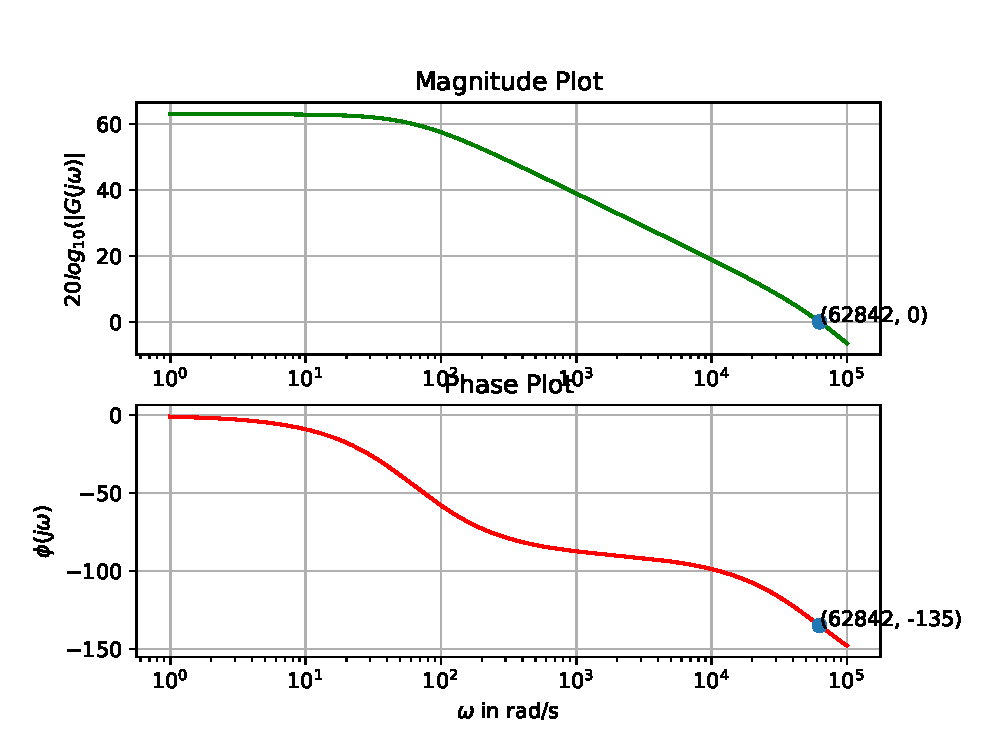
\includegraphics[width=\columnwidth]{./figs/ee18btech11034/ee18btech11034_2.eps}
\caption{}
\label{fig:ee18btech11034_2}
\end{figure}

Below is the code for computations
\begin{lstlisting}
codes/ee18btech11034/ee18btech11034.py
\end{lstlisting}

\item Circuit design for part 1

As given op-amp is in non-inverting configuration and having a pole at $f_{p} = 10$ Hz

The transfer function of op-amp is
\begin{align}
    G_{1}\brak{s} = \frac{10^{5}}{1+\frac{s}{2\pi \times 10}}
\label{eq:ee18btech11034_5}
\end{align}
Required $G(s)$
\begin{align}
    G\brak{s} = G_{1}\brak{s}\frac{1}{1+\frac{s}{2\pi \times 10^{4}}}
\end{align}
So for the error second pole we cascade a RC circuit
\begin{figure}[ht!]
	\begin{center}
		\resizebox{\columnwidth/2}{!}{\begin{circuitikz}[american]
\ctikzset{tripoles/mos style/arrows}
\draw (1,2) to[short, -o] (0,2) node[label={above:$V_{in}$}]{};
\draw (1,2) to[R=$R$, i=$I$] (3,2) to[C=$C$] (3,0) node[ground](GND){};
\draw (3,2) to[short, -o] (4,2) node[label={above:$V_{out}$}]{};
\end{circuitikz}
}
	\end{center}
	\caption{}
	\label{fig:ee18btech11034_figa}
\end{figure}
\begin{align}
\frac{V_{out}}{V_{in}} = \frac{I \times \frac{1}{Cs}}{I \times \brak{R+\frac{1}{Cs}}}
\implies \frac{1}{1+sCR}
\end{align}
Choosing R and C such that
\begin{align}
RC  = \frac{1}{2\pi \times 10^{4}}
\\
\implies 159 \times 10^{-7}
\end{align}
Assuming $R = 5300 \ohm$ and $C=3 \times 10^{-9}F = 3nF$ 

Circuit for open loop transfer function $G\brak{s}$
\begin{figure}[ht!]
	\begin{center}
		\resizebox{\columnwidth}{!}{\begin{circuitikz}[american]

\draw (2,2)  node[op amp] (OA) {};
\draw (OA.+) -- (0,1.5) to[vsourcesin, l= $V_{s}$] (0,0) node[ground](GND){};
\draw (OA.-) -- (0,2.5) node[ground, rotate=270](GND){};
\draw (OA.out) -- (3,2) node[label={above:$V_{p}$}]{};
\draw (3,2) to[R=$5300\ohm$] (5.5,2) node[label={}]{} to[C,l_=$3nF$] (5.5,0) node[ground](GND){};
\draw (5.5,2) -- (6.5,2) node[label={above:$V_{o}$}]{};

\end{circuitikz}
}
	\end{center}
	\caption{}
	\label{fig:ee18btech11034_figb}
\end{figure}

At operational amplifier
\begin{align}
\frac{V_{p}}{V_{s}} = G_{1}\brak{s}
\label{eq:ee18btech11034_6}
\end{align}

At RC circuit
\begin{align}
\frac{V_{o}}{V_{p}} = \frac{1}{1+\frac{s}{2\pi \times 10^{4}}}
\label{eq:ee18btech11034_7}
\end{align}
From \eqref{eq:ee18btech11034_5},\eqref{eq:ee18btech11034_6} and \eqref{eq:ee18btech11034_7}
Open loop gain 
\begin{align}
G = \frac{V_{o}}{V_{s}} = \frac{10^{5}}{\brak{1+\frac{s}{2\pi \times 10}}\brak{1+\frac{s}{2\pi \times 10^{4}}}}
\end{align}

For the feedback gain H
Choose a resistance network such that 
\begin{align}
H = \frac{V_{f}}{V_{o}} = \frac{R_{1}}{R_{1}+R_{2}} \approx 0.01
\end{align}

Choosig R1 and R2 as
\begin{align}
R1 = 10\ohm
\end{align}
\begin{align}
R2 = 1000\ohm
\end{align}

\begin{figure}[ht!]
	\begin{center}
		\resizebox{\columnwidth/2}{!}{\begin{circuitikz}[american]
\ctikzset{tripoles/mos style/arrows}
\draw (1,2) to[short, -o] (0,2) node[label={above:$V_{o}$}]{};
\draw (1,2) to[R=$1000\ohm$] (2,2) -- (3,2) to[R=$10\ohm$] (3,0) node[ground](GND){};
\draw (3,2) to[short, -o] (4,2) node[label={above:$V_{f}$}]{};
\end{circuitikz}
}
	\end{center}
	\caption{}
	\label{fig:ee18btech11034_figc}
\end{figure}
From Fig.\ref{fig:ee18btech11034_figc}
\begin{align}
\frac {V_{f}}{V_{o}} = \frac{10}{10+1000}
\\
\implies \approx 0.01
\end{align}

Circuit for closed loop transfer function 
\begin{figure}[ht!]
	\begin{center}
		\resizebox{\columnwidth}{!}{\tikzstyle{block} = [draw, rectangle, 
    minimum height=1.25em, minimum width=2.5em]
\tikzstyle{sum} = [draw, circle, node distance=1cm]
\tikzstyle{input} = [coordinate]
\tikzstyle{output} = [coordinate]
\tikzstyle{pinstyle} = [pin edge={to-,thin,black}]

% The block diagram code is probably more verbose than necessary
\begin{tikzpicture}[auto, node distance=2.5cm,>=latex']
    % We start by placing the blocks
    \node [input, name=input] {};
    \node [sum, right of=input] (sum) {};
    \node [block, right of=sum] (controller) {$\frac{10^{5}}{\brak{1+\frac{s}{2\pi \times 10}}\brak{1+\frac{s}{2\pi \times 10^{4}}}}$};
    
    % We draw an edge between the controller and system block to 
    % calculate the coordinate u. We need it to place the measurement block. 
   
    \node [output, right of=controller] (output) {};
    \node [block, below of=controller] (measurements) {$1.414 \times 10^{-2}$};

    % Once the nodes are placed, connecting them is easy. 
    \draw [draw,->] (input) -- node[pos=0.99] {$+$} node {$V_{s}$} (sum);
    \draw [->] (sum) -- node {$V_{i}$} (controller);
    \draw [->] (controller) -- node [name=y] {$V_{o}$}(output);
    \draw [->] (y) |- (measurements);
    \draw [->] (measurements) -| node[pos=0.99] {$-$} node [near end] {$V_{f}$} (sum);
\end{tikzpicture}}
	\end{center}
	\caption{}
	\label{fig:ee18btech11034_figd}
\end{figure}

\textbf{The above Fig.\ref{fig:ee18btech11034_figd} is feed back circuit for part 1 of question}

\item Circuit design for part 2

As open loop system is not changed for phase margin to be $45\degree$ we change feedback gain H

Required $H = 1.414 \times 10^{-2}$

Choosing R1 and R2 as
\begin{align}
R1 = 14\ohm
\end{align}
\begin{align}
R2 = 1000\ohm
\end{align}
\begin{align}
H = \frac{R_{1}}{R_{1}+R_{2}}
\\
\implies \frac{14}{14+1000} \approx 1.4 \times 10^{-2}
\end{align}
Circuit for closed loop transfer function 
\begin{figure}[ht!]
	\begin{center}
		\resizebox{\columnwidth}{!}{\begin{circuitikz}[american]

\draw (2,2)  node[op amp] (OA) {};
\draw (OA.+) -- (0,1.5) to[vsourcesin, l= $V_{s}$] (0,0) node[ground](GND){};
\draw (OA.-) -- (0,2.5) node[label={below:$V_{f}$}]{} to[R,l_=$14\ohm$] (-2,2.5) node[ground](GND){};
\draw (OA.out) -- (3,2) node[label={above:$V_{p}$}]{};
\draw (3,2) to[R=$5300\ohm$] (5.5,2) node[label={}]{} to[C,l_=$3nF$] (5.5,0) node[ground](GND){};
\draw (5.5,2) -- (6.5,2) node[label={above:$V_{o}$}]{};
\draw (5.5,2) -- (5.5,4) to[R=$10^{3}\ohm$] (0,4) -- (0,2.5);
\end{circuitikz}
}
	\end{center}
	\caption{}
	\label{fig:ee18btech11034_fige}
\end{figure}

\textbf{The above Fig.\ref{fig:ee18btech11034_fige} is feed back circuit for part 2 of question}

\end{enumerate}
